% overall design, architectural design, interface design, database design
% implementation - frontend (main, canvas, checklist) and backend (template creation, template storing, 3, 4)
% user diagram

\section{Designs}

\begin{figure}[ht]
    \centering
    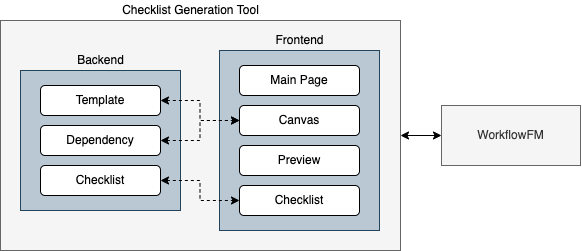
\includegraphics[width=0.8\textwidth]{overleaf/images/system_structure.png}
    \caption{Software's Structure}
    \label{fig:software_structure}
\end{figure}

\subsection{Architectural Design}

\subsection{Interface Design}

- Chen's design \cite{checklistdesign}

- Form creators; e.g. google forms, microsoft forms

\subsection{Database Design}
- main checklist design

- templates, components

- input\_information\_parent, input\_information\_child, input\_information\_child\_query

-

- healthcare

- payment

\begin{figure}[ht]
    \centering
    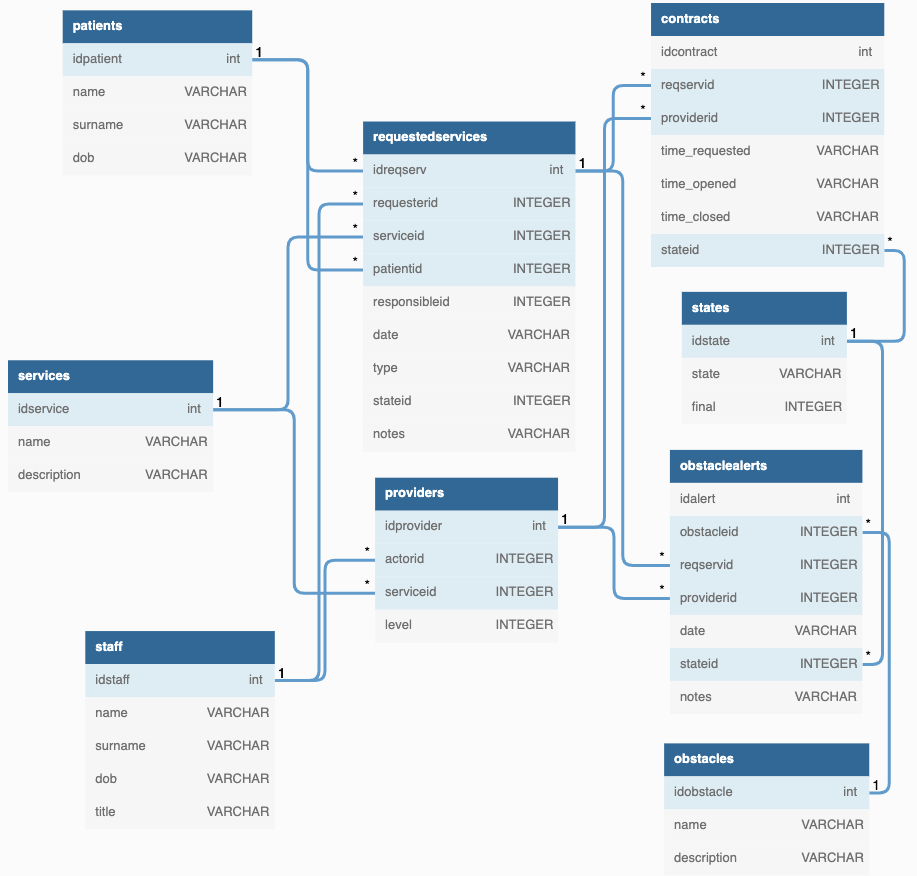
\includegraphics[width=\textwidth]{overleaf/images/chens_healthcare_db_design.png}
    \caption{Chen's Healthcare Database Design}
    \label{fig:chens_healthcare_db_design}
\end{figure}

\begin{figure}[ht]
    \centering
    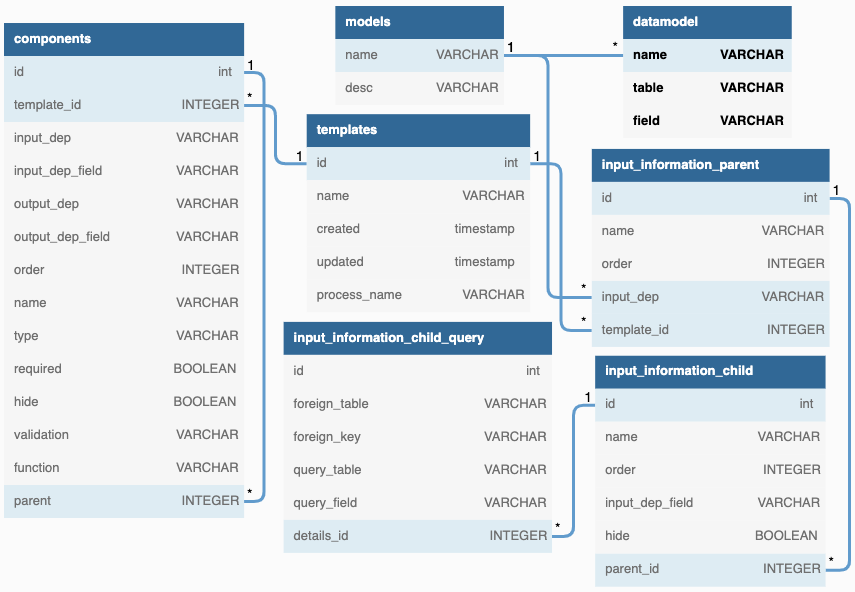
\includegraphics[width=\textwidth]{overleaf/images/checklist_db_design.png}
    \caption{Checklist Database Design}
    \label{fig:checklist_db_design}
\end{figure}

\section{Implementation}
\subsection{Frontend}
- Main screen

- Canvas

- Preview

- Checklist

\subsection{Backend}
- workflow process to checklist template

- get dependencies

- get foreign tables/keys

- saving template

- retrieve finished templates

\section{User Diagrams}

\begin{figure}[ht]
    \centering
    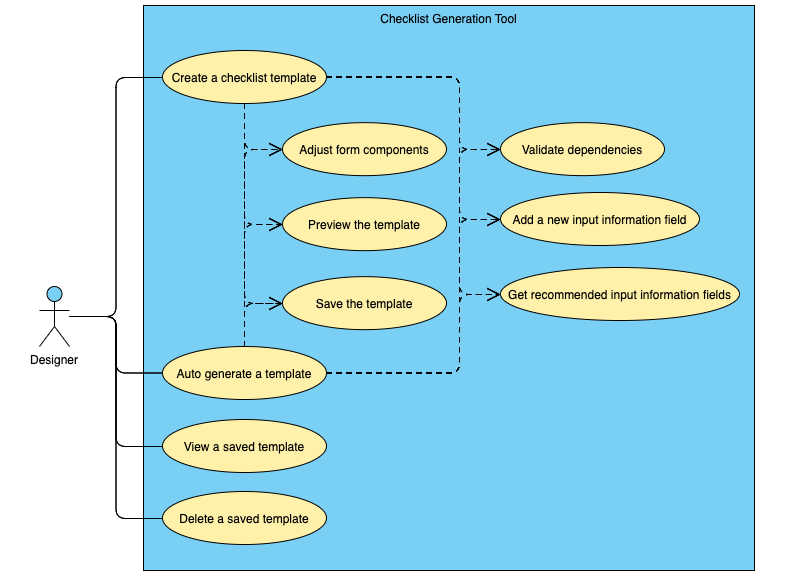
\includegraphics[width=\textwidth]{overleaf/images/use_case_diagram.png}
    \caption{Use Case Diagram}
    \label{fig:use_case_diagram}
\end{figure}
